\documentclass[14pt,final,oneside]{extreport}

\usepackage[a4paper, mag=1000, left=2.5cm, right=1cm, top=2cm, bottom=2cm, headsep=0.7cm, footskip=1cm]{geometry}
% {{{ babel c языковым пакетом не должны быть первым импортируемым пакетом
\usepackage[utf8]{inputenc}
\usepackage[T1,T2A]{fontenc}
\usepackage[russian]{babel}
% }}}

%\usepackage{cmap} %поиск в pdf
\usepackage{amsmath,amsthm,amssymb}
\usepackage{mathtext}
\usepackage{indentfirst}
\usepackage{graphicx}
\graphicspath{{/home/ivan/itmo/informatics/latex}}
\DeclareGraphicsExtensions{.pdf,.png,.jpg}
%\usepackage{bookmark}

\usepackage[dvipsnames]{xcolor}
\usepackage{hyperref} % использование ссылок
\hypersetup{
    colorlinks=true,
    linkcolor=blue,
    filecolor=magenta,      
    urlcolor=magenta,
    %pdftitle={Overleaf Example},
    %pdfpagemode=FullScreen,
}
\usepackage{listings} % использование листингов
\usepackage{caption}
\DeclareCaptionFont{white}{\color{white}} 
\DeclareCaptionFormat{listing}{\colorbox{gray}{\parbox{\textwidth}{#1#2#3}}}
%\captionsetup[lstlisting]{format=listing,labelfont=white,textfont=white}




%\lstset{% настройки вида листинга
%inputencoding=utf8, extendedchars=\true, keepspaces = true, % поддержка кириллицы и пробелов в комментариях
%language=Pascal,            % выбор языка для подсветки (здесь это Pascal)
%basicstyle=\small\sffamily, % размер и начертание шрифта для подсветки кода
%numbers=left,               % где поставить нумерацию строк (слева\справа)
%numberstyle=\tiny,          % размер шрифта для номеров строк
%stepnumber=1,               % размер шага между двумя номерами строк
%numbersep=5pt,              % как далеко отстоят номера строк от подсвечиваемого кода
%backgroundcolor=\color{white}, % цвет фона подсветки - используем \usepackage{color}
%showspaces=false,           % показывать или нет пробелы специальными отступами
%showstringspaces=false,     % показывать илигнет пробелы в строках
%showtabs=false,             % показывать или нет табуляцию в строках
%frame=single,               % рисовать рамку вокруг кода
%tabsize=2,                  % размер табуляции по умолчанию равен 2 пробелам
%captionpos=t,               % позиция заголовка вверху [t] или внизу [b] 
%breaklines=true,            % автоматически переносить строки (да\нет)
%breakatwhitespace=false,    % переносить строки только если есть пробел
%escapeinside={\%*}{*)}      % если нужно добавить комментарии в коде
%}

\sloppy % Решение проблем с переносами (с. 119 Nabor-i...)
\emergencystretch=25pt


%%%%%%%%%%%%%%%%%%%%%%%%%% КОМАНДЫ {Для соответствия ГОСТ}%%%%%%%%%%%%%%%%%%%%%%%%

\newcommand\Chapter[1]{
    \refstepcounter{chapter}
    \chapter*{
        \begin{huge}
        %\textbf{\chaptername\ \arabic{chapter}\\}
        \textbf{\chaptername\ \labnumber\\}
        \end{huge}
        \bigskip \bigskip
        \raggedright #1}
        % Отключена нумерация для chapter в Оглавлении (Содержании):
        %\addcontentsline{toc}{chapter}{\arabic{chapter}. #1}
        \addcontentsline{toc}{chapter}{#1} }

\newcommand\Section[1]{
    \refstepcounter{section}
    \section*{\raggedright
    % Отключена дополнительная нумерация chapter в section в тексте документа:
        %\arabic{chapter}.\arabic{section}. #1}
        \arabic{section}. #1}
    % Отключена дополнительная нумерация chapter в section в Оглавлении (Содержании):
    %\addcontentsline{toc}{section}{\arabic{chapter}.\arabic{section}. #1}
    \addcontentsline{toc}{section}{\arabic{section}. #1} }

\newcommand\Subsection[1]{
    \refstepcounter{subsection}
    \subsection*{\raggedright
        % Отключена дополнительная нумерация chapter в section в тексте документа (можно добавить отступ с помощью \hspace*{12pt}):
        %\arabic{chapter}.\arabic{section}.\arabic{subsection}. #1}
        \arabic{section}. \arabic{subsection}. #1}
        % Отключена дополнительная нумерация chapter в section в Оглавлении (Содержании):
        %\addcontentsline{toc}{subsection}{\arabic{chapter}.\arabic{section}.\arabic{subsection}. #1}
        \addcontentsline{toc}{subsection}{\arabic{subsection}. #1}
}

%\newcommand\Figure[1,2,3]{

        %\refstepcounter{figure}
        %\begin{figure}[h]
            %\center{\includegraphics[width=0.6\linewidth]{#1}}
        %\caption{#2}
        %\label{fig:#3}
    %\end{figure}
%}

%%%%%%%%%%%%%%%%%%%%%%%%%% КОМАНДЫ %%%%%%%%%%%%%%%%%%%%%%%%


\begin{document}


%%%%%%%%%%%%%%%%%%%%%%%%%% ПЕРЕМЕННЫЕ {{{ %%%%%%%%%%%%%%%%%%%%%%%%%%%%
\newcommand\labnumber{3}
\newcommand\student{Тюрин Иван Николаевич} % определение ФИО студента, выполнившего работу
\newcommand\studygroup{P3110} % определение учебной группы студента, выполнившего работу
\newcommand\variant{№ 54}
\newcommand\subject{Информатика}
\newcommand\teacher{Балакшин П. В.,\\
                    Рудникова Т. В.}

\newcommand\labname{Синтез помехоустойчивого кода}
%%%%%%%%%%%%%%%%%%%%%%%%%% }}} ПЕРЕМЕННЫЕ %%%%%%%%%%%%%%%%%%%%%%%%%%%%

% Переоформление некоторых стандартных названий
%\renewcommand{\chaptername}{Лабораторная работа}
\renewcommand{\chaptername}{Лабораторная работа} % переименование глав
\def\contentsname{Содержание} % переименование оглавления


% Оформление титульного листа
\begin{titlepage}

    % Название университета
    \begin{center}
    \textsc{Национальный исследовательский университет ИТМО\\[5mm]
    Факультет программной инженерии и компьютерной техники\\[2mm]
    Кафедра вычислительной техники}

    \vfill
    \vfill
    % Название работы
    \textbf{ОТЧЁТ ПО ЛАБОРАТОРНОЙ РАБОТЕ\\[3mm]
    курса <<\subject>> \\[6mm]
    Вариант \variant
    \\[20mm]
    }
    \end{center}


\hfill
\hfill

    % Информация об авторе работы и проверяющем
    \begin{flushright}
        \begin{minipage}{.5\textwidth}
            
        Выполнил студент:\\[2mm] 
        \student\\[2mm]
        группа: \studygroup\\[5mm]

        Преподаватель:\\[2mm] 
        \teacher

        \end{minipage}%
    \end{flushright}

\vfill

    % Нижний колонтитул первой страницы
    \begin{center}
        Санк-Петербург, \the\year\,г.
    \end{center}

\end{titlepage}


% Содержание
\tableofcontents
\newpage

%%%%%%%%%%%%%%%%%%%%%% КОД РАБОТЫ %%%%%%%%%%%%%%%%%%%%%%%%%%

\Chapter{\labname}

\Section{Задание варианта \variant}

\paragraph{}
Задание 1:
\begin{tabular}{|c||c|c|c|c|c|c|c|}
    \hline
    Вариант & r_1 & r_2 & i_1 & r_3 & i_2 & i_3 & i_4 \\
    \hline
    39 & 1  & 1  & 0  & 0  & 0  & 1  & 0  \\
    \hline
    71 & 0 & 0 & 0 & 0 & 1 & 0 & 1 \\
    \hline
    3 & 0 & 0 & 1 & 1 & 0 & 0 & 0 \\
    \hline
    23 & 1 & 0 & 0 & 1 & 0 & 0 & 1 \\
    \hline

\end{tabular}

\paragraph{}
Задание 2.
\begin{tabular}{|c||c|c|c|c|c|c|c|c|c|c|c|c|c|c|c|}
    \hline
    Вариант & r_1 & r_2 & i_1 & r_3 & i_2 & i_3 & i_4 & r_4 & i_5 & i_6 &  i_7 & i_8 & i_9 & i_{10} & i_{11}\\
    \hline
    39 & 0 & 1 & 0 & 0 & 0 & 1 & 1 & 0 & 1 & 1 & 0 & 0 & 0 & 1 & 1\\
    \hline

\end{tabular}

\paragraph{}
Задание 3.
Принять число 720 как число информационных разрядов в передоваемом сообщении. Вычислить для данного числа минимальное число проверочных разрядов и коэфициент изыточности.

\paragraph{}
Задание 4.
Написать программу на любом языке программирования,
которая на вход из командной строки получает набор из 7 цифр «0» и «1»,
записанных подряд, анализирует это сообщение на основе классического
кода Хэмминга (7,4), а затем выдает правильное сообщение (только информационные биты) и указывает бит с ошибкой при его налиции.


\newpage
\Section{Выполнение задания 1}

    \begin{figure}[h]
        \center{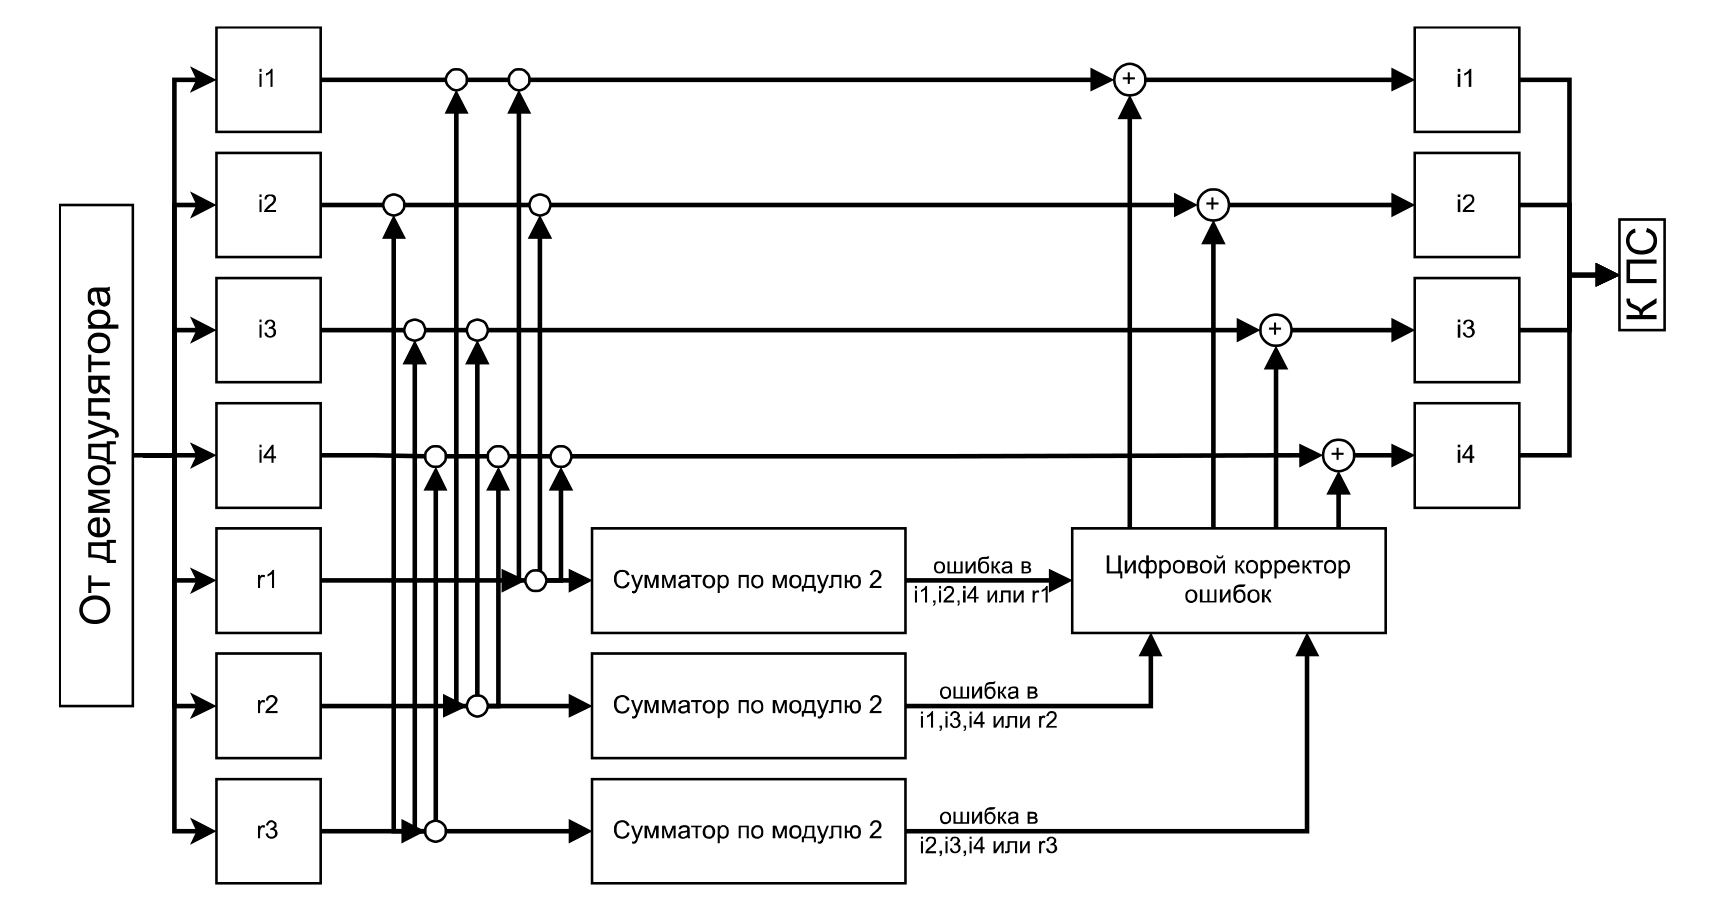
\includegraphics[width=\linewidth]{lab2-inf-7-4.png}}
        \begin{center} \begin{tabular}{|c|c|c|c|c|c|c|c|c|}
                \hline
                    & 1 & 2 & 3 & 4 & 5 & 6 & 7 & \\
                \hline
                2^4 & r_1 & r_2 & i_1 & r_3 & i_2 & i_3 & i_4 & S\\
                \hline
                1 & x & & x & & x & & x  & S_1\\
                2 &  & x & x & & & x& x & S_2\\
                4 &  & & & x& x&x& x& S_3\\
                \hline
            \end{tabular}
        \end{center}
        \caption{Схема декодирования кода Хэмминга}
        \label{fig:7-4}
    \end{figure}

    \Subsection{Вариант 39}
        \begin{tabular}{|c||c|c|c|c|c|c|c|}
            \hline № & r_1 & r_2 & i_1 & r_3 & i_2 & i_3 & i_4 \\
            \hline
            39  & 1 & 1& 0 & 0& 0 & 1 & 0 \\
            \hline
        \end{tabular}\\[2mm]

        \noindent
        Вычислим значение синдрома:\\
        $S_1 = r_1 \otimes i_1 \otimes i_2 \otimes i_4 = 1 \otimes 0 \otimes 0 \otimes 0 = 1$\\
        $S_2 = r_2 \otimes i_1 \otimes i_3 \otimes i_4 = 1 \otimes 0 \otimes 1 \otimes 0 = 0$\\
        $S_3 = r_3 \otimes i_2 \otimes i_3 \otimes i_4 = 0 \otimes 0 \otimes 1 \otimes 0 = 1$\\
        \\\noindent
        $(S_1,\ S_2,\ S_3) = (1,\ 0,\ 1)$ --- 5 позиция, ошибка в символе $i_2$\\[2mm]

        \noindent
        Исходное сообщение: 1100110 

    \Subsection{Вариант 71}
        \begin{tabular}{|c||c|c|c|c|c|c|c|}
            \hline
            № & r_1 & r_2 & i_1 & r_3 & i_2 & i_3 & i_4 \\
            \hline
            71  & 0 & 0& 0 & 0& 1 & 0 & 1 \\
            \hline
        \end{tabular}\\[5mm]

        \noindent
        Вычислим значение синдрома:\\
        $S_1 = r_1 \otimes i_1 \otimes i_2 \otimes i_4 = 0 \otimes 0 \otimes 1 \otimes 1 = 0$\\
        $S_2 = r_2 \otimes i_1 \otimes i_3 \otimes i_4 = 0 \otimes 0 \otimes 0 \otimes 1 = 1$\\
        $S_3 = r_3 \otimes i_2 \otimes i_3 \otimes i_4 = 0 \otimes 1 \otimes 0 \otimes 1 = 0$\\
        
        \noindent
        $(S_1,\ S_2,\ S_3) = (0,\ 1,\ 0)$ --- 2 позиция, ошибка в символе $r_2$\\[2mm]

        \noindent
        Исходное сообщение: 0100101 

    \Subsection{Вариант 3}
        \begin{tabular}{|c||c|c|c|c|c|c|c|}
            \hline
            № & r_1 & r_2 & i_1 & r_3 & i_2 & i_3 & i_4 \\
            \hline
            3  & 0 & 0 & 1 & 1& 0 & 0 & 0 \\
            \hline
        \end{tabular}\\[5mm]

        \noindent
        Вычисляем значение синдрома:\\
        $S_1 = r_1 \otimes i_1 \otimes i_2 \otimes i_4 = 0 \otimes 1 \otimes 0 \otimes 0 = 1$\\
        $S_2 = r_2 \otimes i_1 \otimes i_3 \otimes i_4 = 0 \otimes 1 \otimes 0 \otimes 0 = 1$\\
        $S_3 = r_3 \otimes i_2 \otimes i_3 \otimes i_4 = 1 \otimes 0 \otimes 0 \otimes 0 = 1$\\
        
        \noindent
        $(S_1,\ S_2,\ S_3) = (1,\ 1,\ 1)$ --- 7 позиция, ошибка в символе $r_1$\\[2mm]
        \noindent
        Исходное сообщение: 0011001    


    \Subsection{Вариант 23}
        \begin{tabular}{|c||c|c|c|c|c|c|c|}
            \hline
            № & r_1 & r_2 & i_1 & r_3 & i_2 & i_3 & i_4 \\
            \hline
            23  & 1 & 0& 0 & 1 & 0 & 0 & 1 \\
            \hline
        \end{tabular}\\[5mm]

        \noindent
        Вычисляем значение синдрома:\\
        $S_1 = r_1 \otimes i_1 \otimes i_2 \otimes i_4 = 1 \otimes 0 \otimes 0 \otimes 1 = 0$\\
        $S_2 = r_2 \otimes i_1 \otimes i_3 \otimes i_4 = 0 \otimes 0 \otimes 0 \otimes 1 = 1$\\
        $S_3 = r_3 \otimes i_2 \otimes i_3 \otimes i_4 = 1 \otimes 0 \otimes 0 \otimes 1 = 0$\\

        \noindent
        $(S_1,\ S_2,\ S_3) = (0,\ 1,\ 0)$ --- 2 позиция, ошибка в символе $r_2$\\[2mm]
        \noindent
        Исходное сообщение: 1101001

\newpage
\Section{Выполнение задания 2}

    \begin{figure}[h]
        \center{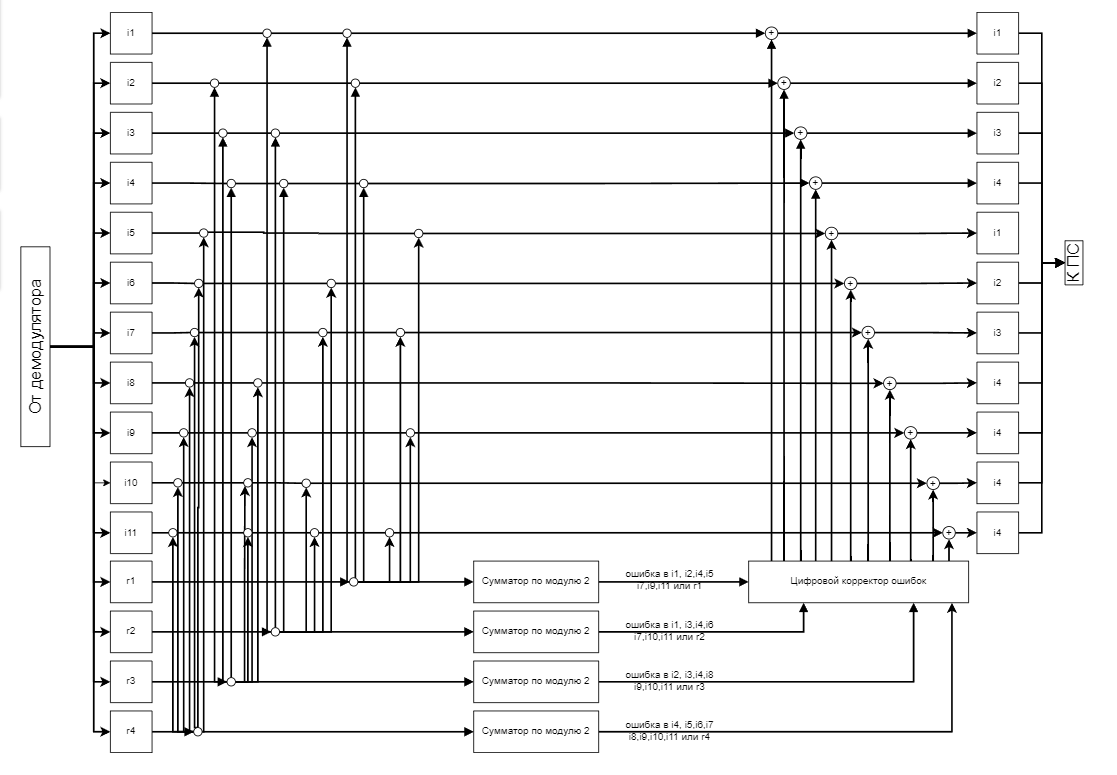
\includegraphics[width=\linewidth]{lab2-inf-15-11.png}}
    \begin{center} 
        \begin{tabular}{|c|c|c|c|c|c|c|c|c|c|c|c|c|c|c|c|c|}
            \hline
                & 1 & 2 & 3 & 4 & 5 & 6 & 7 & 8 & 9 & 10 & 11 & 12 & 13 & 14 & 15 &\\
            \hline
            2^4 & r_1 & r_2 & i_1 & r_3 & i_2 & i_3 & i_4 & r_4 & i_5 & i_6 & i_7 & i_8 & i_9 & i_{10} & i_{11} & S\\
            \hline
            1 &x& &x& &x& &x& &x& &x& &x& &x&S_1\\
            2 & &x&x& & &x&x& & &x&x& & &x&x&S_2\\
            4 & & & &x&x&x&x& & & & &x&x&x&x&S_3\\
            8 & & & & & & & &x&x&x&x&x&x&x&x&S_4\\
            \hline
        \end{tabular}
    \end{center}
        \caption{Схема декодирования кода Хэмминга}
        \label{fig:15-11}
    \end{figure}


    \begin{tabular}{|c||c|c|c|c|c|c|c|c|c|c|c|c|c|c|c|}
        \hline
        № & r_1 & r_2 & i_1 & r_3 & i_2 & i_3 & i_4 & r_4 & i_5 & i_6 &  i_7 & i_8 & i_9 & i_{10} & i_{11}\\
        \hline
        39 & 0 & 1 & 0 & 0 & 0 & 1 & 1 & 0 & 1 & 1 & 0 & 0 & 0 & 1 & 1\\
        \hline
    \end{tabular}
    \\[5mm]

    \noindent
    Вычисляем значение синдрома:\\
    $S_1 = r_1 \otimes i_1 \otimes i_2 \otimes i_4 \otimes i_5 \otimes i_7 \otimes i_9 \otimes i_{11} = 
         0 \otimes 0 \otimes 0 \otimes 1 \otimes 1 \otimes 0 \otimes 0 \otimes 1 = 1$\\
    $S_2 = r_2 \otimes i_1 \otimes i_3 \otimes i_4 \otimes i_6 \otimes i_7 \otimes i_{10} \otimes i_{11} =
         1 \otimes 0 \otimes 1 \otimes 1 \otimes 1 \otimes 0 \otimes 1 \otimes 1 = 0$\\
    $S_3 = r_3 \otimes i_2 \otimes i_3 \otimes i_4 \otimes i_8 \otimes i_9 \otimes i_{10} \otimes i_{11} =
        0 \otimes 0 \otimes 1 \otimes 1 \otimes 0 \otimes 0 \otimes 1 \otimes 1 = 0$\\
    $S_4 = r_4 \otimes i_5 \otimes i_6 \otimes i_7 \otimes i_8 \otimes i_9 \otimes i_{10} \otimes i_{11} = 
    0 \otimes 1 \otimes 1 \otimes 0 \otimes 0 \otimes 0 \otimes 1 \otimes 1 = 0$\\

        \noindent
        $(S_1,\ S_2,\ S_3,\ S_4) = (1,\ 0,\ 0,\ 0)$ --- ошибка в 1 символе.\\[2mm]
        
        Исходное сообщение: 110001101100011

\Section{Выполнение задания 3}
Вычислить для числа 720 минимальное число проверочных разрядов и коэфициент избыточности.\\
По формуле: $2^r\geqslant 720+r+1$\\[2mm]
$r=9:\ 512<720+9+1$ --- недостаточно;\\
$r=10:\ 1024>720+10+1$ --- достаточно.\\[2mm]
Количесво проверочных разрядов --- $r=\bf{10}$\\
Общее колиичество бит: $n=r+i=10+720=730$\\
Коэфициент избыточности: $k=\cfrac r n = \cfrac {11} {730} \approx 0.0137$\\

\Section{Выполнение задания 4}
Была написана программа на языке программирования Python, которая на вход из командной строки получает набор из 7 цифр <<0>> и <<1>>, записанных подряд, анализирует это сообщение на основе классического кода Хэмминга (7,4), а затем выдаёт правильное сообщение (только информационные биты) и указывает бит с ошибкой при его наличии.\\

Исходный код программы размещен в личном удаленном репозитории. Её исходный код можно найти по ссылке: \url{https://github.com/e1turin/itmo-informatics/blob/main/lab-2/script.py}.



\Section{Вывод}
Научился работать с кодом Хэмминга, находить ошибки в сообщении и исправлять их. Узнал, как найти минимальное количество проверочных разрядов и коэффициент избыточности. Написал программу, реализующую код Хэмминга.\\
\newpage


%%%%%%%%%%%%%%%%%%%% СПИСОК ЛИТЕРАТУРЫ {{{ %%%%%%%%%%%%%%%%%%%%%
%\Section{Список литературы}
% Для отчёта он не обязателен
\bibliographystyle{plain}

\begin{thebibliography}{3}
    \addcontentsline{toc}{chapter}{Список лиетратуры}

    \bibitem{gutgut:1}
    Код Хэмминга. Пример работы алгоритма. URL: \url{https://habr.com/ru/post/140611/};

    \bibitem{gutgut:2}
    Избыточное кодирование, код Хэмминга. URL: \url{https://neerc.ifmo.ru/wiki/index.php?title=%D0%98%D0%B7%D0%B1%D1%8B%D1%82%D0%BE%D1%87%D0%BD%D0%BE%D0%B5_%D0%BA%D0%BE%D0%B4%D0%B8%D1%80%D0%BE%D0%B2%D0%B0%D0%BD%D0%B8%D0%B5,_%D0%BA%D0%BE%D0%B4_%D0%A5%D1%8D%D0%BC%D0%BC%D0%B8%D0%BD%D0%B3%D0%B0}.

\end{thebibliography}

%%%%%%%%%%%%%%%%%%%% }}} СПИСОК ЛИТЕРАТУРЫ %%%%%%%%%%%%%%%%%%%%%
\end{document}
